\vbtitle[\LARGE]{Limits}
\addcontentsline{toc}{section}{Limits}


\vbdefinition{
Imagine you live in a society where theft is a serious crime. One day, you steal something and flee to an unknown city. The police start their investigation by questioning your family, who say, "He has gone to Delhi." Then they question your friends, who say, "He has gone to Mumbai." With these conflicting reports, the police don't know where to look and can't determine your exact location.\\[2mm]
In mathematics, this situation is similar to finding the limit of a function as it approaches a particular point. Your location represents the value the function is approaching.\\[2mm]
If your family and friends (the function's behavior from different directions) provide conflicting reports (different values), the police (mathematicians) can't determine a single location (the limit doesn't exist). For a limit to exist, both sides need to agree on the same city (value).\\[2mm]
So, just as the police need consistent reports to find you, a limit in math requires the function to approach the same value from all directions.\\[2mm]
\textbf{In mathematics, for functions that do not provide finite outputs directly or give conflicting outputs, we use limits to investigate their behavior and determine their potential outputs.}\\
}



\vbdefinition{Suppose that a function $f(x)$ approaches a value $m$ as $x$ approaches $a$. Then the limit of $f(x)$ as $x$ tends to $a$, is $m$.
It is denoted as 
\[ 
\lim_{x \to a}f(x)=m
\]
$x \to a$ denotes `$x$ tends to $a$'.
Whenever we say `$x$ tends to $a$' or `$x$ approaches $a$', it means $x$ is very close to $a$, but, it is never equal to $a$.
}

\begin{enumerate}
    \item[Q. ] Let $f(x)=x$\\What is the limit of $f(x)$ as $x \to a$?
        \begin{center}
            \begin{tikzpicture}
                \draw[<->] (-5,0)--(5, 0) node[below right]{\textit{x-axis}};
                \draw (0, 0) node{$\bullet$};
                \draw (0, 0) node[below]{$a$};
                \draw[->] (-1.5,0.5)--(-0.2, 0.5) node[above left]{$x \to a-0$};
                \draw[->] (1.5,0.5)--(0.2, 0.5) node[above right]{$a+0 \leftarrow x$};
            \end{tikzpicture}
        \end{center}
        \vbdefinition{
            \begin{align*}
                \intertext{$x$, can approach a real number $a$ from two sides-left hand side (i.e., always being smaller than $a$) and right hand side (i.e., always being greater than $a$)}
                x &\to a-0\\
                \intertext{denotes that $x$ approaches $a$ from left}
                x &\to a+0\\
                \intertext{denotes that $x$ approaches $a$ from right.}
                \intertext{As $x$ approaches $a$ from left, $f(x)$ approaches $a$ because $f(x)=x$.}
                \intertext{i.e.,}
                \lim_{x \to a-0}f(x)&=a\\
                \intertext{On the other hand, as $x$ approaches $a$ from right, $f(x)$ approaches $a$ because $f(x)=x$.}
                \intertext{i.e.,}
                \lim_{x \to a+0}f(x)&=a
                \intertext{\textbf{Existence of limit:}}
                \intertext{We say that $\underset{x \to a}{\lim}~f(x)$ exists if}
                \lim_{x \to a-0} f(x) = \lim_{x \to a+0} f(x) &= a \qquad\textit{(finite real number)}\\
                \intertext{$\underset{x \to a-0}{\lim}~f(x)$ and $\underset{x \to a+0}{\lim}~f(x)$ are called left hand limit and right hand limit respectively of function $f(x)$ at $x=a$.}
            \end{align*}
            }
\end{enumerate}



\vbsubtitle{Some Important Results}\\[2mm]
\hspace*{10mm}Let 
 $\underset{x \to a}\lim ~f(x)= l$ ~and~ 
 $\underset{x \to a}\lim ~g(x) = m$, where $l$ and $m$ are finite real numbers.\\
\begin{enumerate}[label=\textit{(\alph*)}]
\item $\underset{x \to a}\lim ~[f(x) \pm g(x)] = l \pm m$
\item $\underset{x \to a}\lim ~[f(x) \cdot g(x)] = l \cdot m$
\item $\underset{x \to a}\lim ~\left[\dfrac{f(x)}{g(x)}\right] = \dfrac{l}{m}$,~~\textit{provided} $m \neq 0$\\[4 mm]
\end{enumerate}

\vbsubtitle{Some Limits Involving Trigonometric Functions}
\begin{enumerate}[label=\textit{(\roman*)}]
\item $\underset{x \to 0}\lim ~ \sin x = 0$
\item $\underset{x \to 0}\lim ~ \cos x = 1$
\item $\underset{x \to 0}\lim ~ \tan x = 0$
\item $\underset{\theta \to 0}\lim ~ \frac{\sin \theta}{\theta} = 1$\\[2 mm]
\textit{\textbf{Proof : }}\\


\begin{tikzpicture}[scale=0.8]
    \draw[->] (-3, 0)--(5, 0);
    \draw[->] (1, -4)--(1, 4);
    \draw (1, 0) node[below left]{O} circle[radius=2.5] (3.5, 0) node[below right]{$A$};
    \draw (1, 0)--([turn]45:2.5)--(3.5, 0);
    \draw (1.5, 0) arc[start angle=0, end angle=45, radius=0.5] node[right]{$\theta$};

    \draw (3.3, 2.1) node {$B$};
    \draw (3.65, 1.1) node {$P$};
    \draw (1.8, 1) node[above]{$R$};

    \node [right] at (-10, 5.2){Area of $\triangle OAB = \frac{1}{2}R^2 \sin \theta$};
    \node [right] at (-10, 4.2){Area of sector $OAPB = \frac{1}{2}\theta R^2$};

    \node [right, text width= 7 cm] at (-13, 1.6){As $\theta \to 0$, side $AB$ and arc $APB$ tends to coincide with each other. Thus, as $\theta \to 0$, area of $\triangle OAB$ tends to be equal to the area of sector $OAPB$.};

    %\node [below left,text width=6cm, align=justify] at (-5,5) {
    %\par{Area of $\triangle OAB = \frac{1}{2}R^2 \sin \theta$\\
    %}};

    \node [right, text width= 7 cm] at (-10, -1.8){\[ \underset{x \to 0}\lim \left( \frac{\frac{1}{2}R^2\sin \theta}{\frac{1}{2}\theta R^2} \right)=1  \]};

    \node [right, text width= 7 cm] at (-10, -3.7){\[ \underset{x \to 0}\lim ~\frac{\sin \theta}{\theta}=1  \]};
    \node [right, text width= 7 cm] at (-10, -5){Note that $\theta$ is in radian.};
\end{tikzpicture}

\item $\underset{x \to 0}\lim ~ {\frac{\tan x}{x}} = 1$\\[2.5 mm]
\textit{\textbf{Proof : }}\\

\begin{align*}
\underset{x \to 0}\lim ~ {\frac{\tan x}{x}} & = \underset{x \to 0}\lim ~ \left(\frac{\sin x}{x}\right) \left(\frac{1}{\cos x}\right)\\[2 mm]
& = \underset{x \to 0}\lim ~ \left(\frac{\sin x}{x}\right) \cdot \underset{x \to 0}\lim ~\left(\frac{1}{\cos x}\right)\\[2 mm]
& = 1 \cdot 1\\
& = 1
\end{align*}

\end{enumerate}

% \pagebreak

% \vbsubtitle{Some Limits Involving Powers}


% \begin{enumerate}[label=(\roman*)]
%     \item $\underset{x \to a}\lim ~ x^m = a^m$  (a, m $\in$ R)\\[2 mm]
%     \item $\underset{x \to a}\lim ~ p^x = p^a$  (a, p $\in$ R)\\[2 mm]
%     \item $\underset{x \to a}\lim ~ \left(1 + \frac{1}{x}\right)^x = e$\\[2 mm]
% \end{enumerate}

% \vbsubtitle{L'Hospital's Rule}\\
% L'Hospital's Rule tells us that if we have an indeterminate form $\frac{0}{0}$ or $\frac{\infty}{\infty}$ all we need to do is differentiate the numerator and differentiate the denominator and then take the limit.

% \[
% \underset{x \to a}\lim ~ \frac{f(x)}{g(x)} = \frac{0}{0} ~~~ \textit{or} ~~~ \underset{x \to a}\lim ~ \frac{f(x)}{g(x)} = \frac{\pm \infty}{\pm \infty}
% \]\\

% Where $a$ can be any real number, infinity or negative infinity.  In these cases we have,\\[2 mm]
% \[
% \underset{x \to a}\lim ~ \frac{f(x)}{g(x)} = \underset{x \to a}\lim ~ \frac{f'(x)}{g'(x)}
% \]
